\documentclass[12pt, a4paper, oneside]{ctexbook}
\usepackage{amsmath, amsthm, amssymb, bm, graphicx, hyperref, mathrsfs}
\usepackage{geometry}
\usepackage{subfigure}
\usepackage{hyperref}[colorlinks=true,linkcolor=black,citecolor=blue,urlcolor=blue]

%设置引用格式
\hypersetup{
	colorlinks=true,linkcolor=black,colorlinks=true,linkcolor=black,citecolor=blue,urlcolor=blue
}
%在LateX中,参考文献的引用一般有两种方式,平 齐 时 用 命 令\cite{...}, 上 标 时用\textsuperscript{\cite{...}}

\CTEXsetup[format={\Large\bfseries}]{section}	%section 居左(默认居中)
\CTEXsetup[format={\huge\bfseries}]{chapter}	%chapter 居左(默认居中)



%配置纸张边缘
\geometry{left=2.54cm,right=2.54cm,top=3.18cm,bottom=3.18cm}


\title{{\Huge{\textbf{RTL模块设计说明文档}}}\normalsize{\\——第六届全国大学生集成电路创新创业大赛景嘉微杯初赛提交文档}}
\author{队名:虹ヶ咲学园芯片设计同好会\\ 成员:黄金源\space邓立唯\space林明锋}
\date{\today}
\linespread{1.5}


\begin{document}
	%-----------------------封面------------------
	\maketitle	
	\pagenumbering{Roman}
	\setcounter{page}{1}
	%-----------------------前言------------------
	\begin{center}
		\Huge\textbf{前言}
	\end{center}~\
	
	本文档(RTL模块设计说明文档)仅作为虹ヶ咲学园芯片设计同好会(成员:黄金源、邓立唯、林明锋)参加第六届全国大学生集成电路创新创业大赛景嘉微杯赛初赛提交文档供评委评分使用。
	~\\
	\begin{flushright}
		\begin{tabular}{c}
			虹ヶ咲学园芯片设计同好会\\
			\today
		\end{tabular}
	\end{flushright}
	%-----------------------目录------------------
	\newpage
	\pagenumbering{Roman}	%Roman or arabic
	\setcounter{page}{1}
	\tableofcontents
	\newpage
	\setcounter{page}{1}
	\pagenumbering{arabic}
	
	%-----------------------正文----------------	
	\chapter{概要}
	上采样 IP 设计采用了模块化设计,主要分为三大部分:
	\begin{enumerate}
		\item Bicubic 上采样模块
		\item 纹理分类模块
		\item 自适应锐化模块
	\end{enumerate}
	
	\begin{figure}[h]
		\centering
		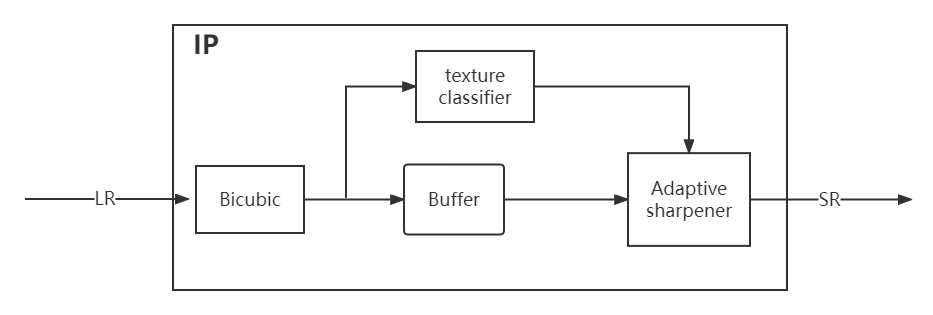
\includegraphics[scale=0.5]{pic/IP-overview}
		\caption{IP 概览}
		\label{fig:ip-overview}
	\end{figure}
	
	\chapter{上采样模块}
	具体说明详见附件文档\href{run:./pic/APV21B_Bicubic_Super_Resolution_IP_UM.pdf}{APV21B\_Bicubic\_Super\_Resolution\_IP\_UM}第四部分具体设计结构。
	
	\chapter{纹理分类模块}
	纹理分类 IP 可提供对于单通道图像每个 $5\times5$ 或 $3\times3$ 图像块的纹理特征进行实时分类。包含了一个归一化高斯卷积核、一个标准拉普拉斯算子、一个 LBP 分类器、三个行缓冲模块、一个滤波器参数存储单元和一个控制单元。为了确保卷积操作后仍需令图像保持原始尺寸,行缓冲模块包含了图像填充处理操作与数据映射模块,由控制单元进行管理。
	%图片
	\section{运算位宽与量化}
	为了节省片上资源的消耗,最大化提升 DSP 利用率,在本模块中,不同部分对于 DSP48E2 均有不同程度上的优化。其中,针对高斯滤波卷积中,将核内权重进行9位无符号量化,在保证高斯卷积核性能的同时充分利用了 DSP48E2 单元的乘法器。这种量化方法仅支持8位图像输入。另外,为了保证后续拉普拉斯滤波数据误差尽可能降低,我们将高斯滤波后的数据量化为20位,尽可能保留数据位宽,避免引入过大误差影响后续操作。在完成拉普拉斯算子卷积后生成的是1位图像输出至 LBP 分类器。
	\section{高斯卷积核}
	高斯卷积核包含了一个高斯系数寄存器单元、一组并行乘法器单元、一组并行的加法器单元、一组并行舍入单元。
	%图片
	每个像素进行高斯滤波卷积是以像素本身为中心,边缘 $5\times5$ 的像素块作为数据输入。每个像素块需要与对应的高斯系数进行相乘然后累和。该高斯卷积核 IP 每个时钟周期处理4个像素。
	\section{高斯系数寄存器单元}
	高斯滤波卷积核系数是由 $\delta$ 所决定,在运行过程中, $\delta$ 不会发生改变,所以该系数为常数。同时,$5\times5$ 卷积核系数与所在卷积核的位置有关系,并且成对应关系。25个系数只需要存6个系数即可。
	%图片
	\section{并行乘法器单元}
	并行乘法单元包含了7个 DSP48E2 用于实现 $5\times5$ 大小的卷积乘法操作。在两个时钟周期内可输出结果(一周期内也可实现结果输出,但为了提升 IP 最大时钟频率,输出端插入一级寄存器增大时序违例余量)\par 由于高斯系数具有对称性,当计算图像块对应的位置的时候,存在几对像素所相乘同一个高斯权重系数。例如上图(0,0)、(0,4)、(4,0)、(4,4)对应像素均是乘以同一个系数。因此,我们可以利用这一特性,并结合 DSP48E2 的大位宽乘法器,同时进行两个8位数据乘以一个9位权重,并保留完整位宽输出。具体设计分析可以查看[APV21B\_Bicubic\_Super\_Resolution\_IP\_UM] 第四部分Biubic设计详细解释中的乘加单元(MA Unit)介绍。%图片引用
	%图片
	\section{拉普拉斯卷积核}
	\section{LBP分类器}
	\section{行缓冲模块}
	
	
	
\end{document}